% Provenance (never printed): enseignement scientifique premiere (2019),
% "Le Soleil, notre source d'energie" (power received by latitude and
% season, albedo, the Earth's radiative balance, the small share stored by
% photosynthesis) and the old seconde/premiere S material on the
% atmosphere's energy; see sources/book2/PROVENANCE.md. Every insolation
% value, budget closure and photosynthesis figure is computed in
% figdata/grade-10/energy_budget.py; the budget fluxes are AR6 WG1
% Figure 7.2.
\chapter{O balanço de energia da Terra}\label{ch:g10:earth-energy-budget}

No dia mais longo do ano, o Sol nunca se põe no Polo Norte. Ele dá a volta
no céu o dia inteiro à mesma altura, cerca de \qty{23}{\degree} acima do
horizonte, e o topo da atmosfera acima do polo recebe num só dia mais luz
solar por metro quadrado do que qualquer outro lugar da Terra ---
\qty{13.0}{kWh}, contra \qty{9.5}{kWh} acima do equador. E, no entanto, o
mar em torno do polo continua coberto de gelo durante todo o verão. Ao
longo de um ano inteiro, por outro lado, o equador recebe duas vezes e meia
mais luz solar que o polo, e os trópicos ficam quentes o ano todo. Este
capítulo acompanha a energia da luz do Sol: quanto chega, onde e quando;
quanto é refletido diretamente de volta para o espaço; como o resto se
reparte entre o ar e o chão, é levado dos trópicos para os polos e
finalmente devolvido ao espaço como luz infravermelha --- e que parte
minúscula dele acaba armazenada pelos seres vivos.
% ledger: earth:TSI, earth:obliquity (daily totals computed in figdata/grade-10/energy_budget.py)

\begin{omfigure}
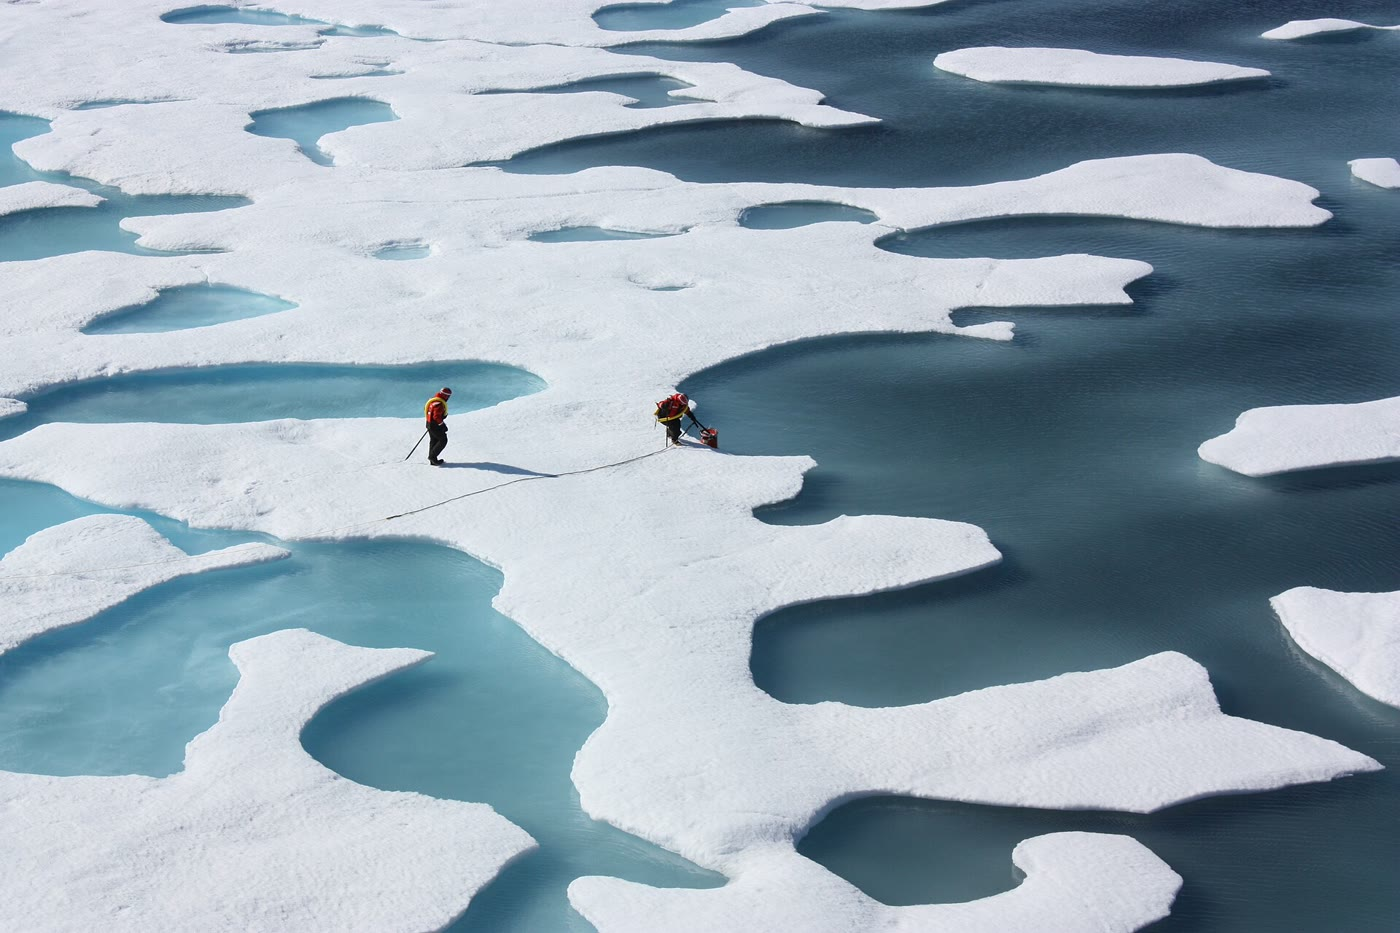
\includegraphics[width=0.78\linewidth]{images/book2/g10-nasa-melt-ponds.jpg}

{\small Gelo marinho no oceano Glacial Ártico em julho, sob um Sol que não
se põe: gelo branco, poças de água de degelo na sua superfície e o mar
aberto, escuro, entre os blocos. Dois cientistas coletam amostras das
poças. Fotografia: NASA Goddard Space Flight Center, 2011 (domínio
público).}
\end{omfigure}

\begin{recall}
As estações vêm da inclinação do eixo da Terra, \qty{23.44}{\degree} em
relação à perpendicular ao plano da sua órbita: em junho, o hemisfério
norte se inclina na direção do Sol, que sobe mais alto no céu e fica mais
tempo acima do horizonte (os livros de física e o Livro 1). A irradiância à
distância da Terra, $S_0 = \qty{1361}{W/m^2}$, o \omterm{def:g10:earth-energy-budget:albedo}{albedo} de Bond de um
planeta e a sua \omterm{def:g10:habitable-planet:equilibrium-temperature}{temperatura de equilíbrio} foram vistos no
\cref{ch:g10:habitable-planet}. Os gases de efeito estufa absorvem parte do
infravermelho emitido pela superfície (os livros de química). O ar quente
sobe e o ar frio desce, o que põe o ar a girar em células de convecção e
move os ventos globais (Livro 1, 8º ano). Plantas, algas e algumas
bactérias fabricam açúcares a partir do gás carbônico e da água com a
energia da luz: é a fotossíntese (os livros de biologia).
\end{recall}

\section{A luz solar recebida}

Vista do Sol, a Terra é um disco. A cada segundo, ela intercepta a luz
solar que cai sobre um disco de raio $R$, o seu próprio raio; mas essa luz
se reparte entre todos os pontos de uma esfera, metade dos quais está na
noite.

\begin{proposition}[Um quarto da constante solar]\label{prop:g10:earth-energy-budget:quarter}
Em média sobre toda a superfície da Terra e sobre o dia e a noite, a
potência da luz solar que chega ao topo da atmosfera é
\[
  \frac{S_0}{4} = \frac{1361}{4} \approx \qty{340}{W/m^2}.
\]
\end{proposition}

\begin{proof}
A Terra intercepta a luz solar que atravessa um disco de área $\pi R^2$
perpendicular aos raios, isto é, uma potência $S_0\,\pi R^2$. Espalhada pela
área da esfera, $4\pi R^2$, isso dá $S_0\,\pi R^2/(4\pi R^2) =
S_0/4$ por metro quadrado.
\end{proof}
% ledger: earth:TSI, ipcc:budget-toa

\begin{omfigure}
\begin{tikzpicture}[font=\small, >={Stealth[length=2mm]}]
  \foreach \y in {-1.2,-0.8,...,1.21}
    \draw[->, omProp!80!black] (-3.4,\y) -- (-1.75,\y);
  \node[anchor=south, font=\footnotesize, align=center] at (-2.6,1.35) {luz solar,\\$S_0$ por m$^2$};
  \draw[fill=omProp!15, draw=omProp!80!black] (-1.6,0) ellipse (0.18 and 1.3);
  \node[anchor=north, font=\footnotesize, align=center] at (-1.6,-1.4) {disco\\$\pi R^2$};
  \shade[ball color=omDef!35] (1.2,0) circle (1.3);
  \fill[black, opacity=0.35] (1.2,1.3) arc (90:-90:1.3) arc (-90:90:0.35 and 1.3);
  \draw[omDef!80!black] (1.2,0) circle (1.3);
  \draw[dashed, black!50] (1.2,-1.3) arc (-90:90:0.35 and 1.3);
  \draw[<->] (1.2,0) -- node[above, font=\footnotesize] {$R$} (2.5,0);
  \node[anchor=west, font=\footnotesize, align=left] at (2.8,0.7) {esfera $4\pi R^2$:\\metade de dia,\\metade de noite};
  \node[anchor=west, font=\footnotesize, align=left] at (2.8,-0.75) {média:\\$S_0\pi R^2/4\pi R^2 = S_0/4$};
\end{tikzpicture}

{\small A Terra intercepta a luz solar que cai sobre um disco do seu próprio
raio, mas a reparte pela área quatro vezes maior de uma esfera: em média,
cada metro quadrado do topo da atmosfera recebe um quarto da constante
solar.}
\end{omfigure}

A média esconde grandes diferenças de um lugar para outro. Um feixe de luz
solar que atinge o chão de modo oblíquo se espalha por uma área maior que um
feixe que o atinge de frente.

\begin{proposition}[A luz solar numa superfície horizontal]\label{prop:g10:earth-energy-budget:height}
Quando o Sol está a uma altura $h$ acima do horizonte, um metro quadrado
horizontal no topo da atmosfera recebe a potência $S_0 \sin h$.
\end{proposition}

\begin{proof}
Tome um feixe de luz solar de seção quadrada de \qty{1}{m^2}, que
transporta $S_0$. No chão, o seu traço é um retângulo com um lado de
\qty{1}{m} e o outro de comprimento $\ell$ ao longo da inclinação dos raios.
No triângulo retângulo formado por esse lado, o raio e a seção do feixe, o
ângulo junto ao chão é $h$ e $\sin h = 1/\ell$. A potência do feixe se
espalha por $\ell$ metros quadrados: $S_0/\ell = S_0 \sin h$ por metro
quadrado.
\end{proof}

\begin{omfigure}
\begin{tikzpicture}[font=\small, >={Stealth[length=2mm]}]
  \fill[omExo!15] (-0.3,-0.5) rectangle (6.3,0);
  \draw[thick] (-0.3,0) -- (6.3,0);
  \foreach \s in {0,0.3,...,1.21}
    \draw[->, omProp!80!black] ({0.6+\s/sin(35)+3.2*cos(35)},{3.2*sin(35)}) -- ({0.6+\s/sin(35)+0.02*cos(35)},{0.02*sin(35)});
  \draw[omProp!80!black, thick] (0.6,0) -- ({0.6+1.2/sin(35)},0);
  \draw (0.6,0) ++(1.6,0) arc (0:35:1.6);
  \node[font=\footnotesize] at ({0.6+1.85*cos(17)},{1.85*sin(17)}) {$h$};
  \draw[<->] (0.6,-0.25) -- node[below, font=\footnotesize] {$\ell = 1/\sin h$} ({0.6+1.2/sin(35)},-0.25);
  \node[anchor=south west, font=\footnotesize, align=left] at (4.35,1.95) {feixe de\\seção\\\qty{1}{m^2}};
\end{tikzpicture}

{\small Luz solar que chega a uma altura $h$ acima do horizonte: o mesmo
feixe cobre $1/\sin h$ metros quadrados de chão horizontal, logo cada metro
quadrado recebe $S_0 \sin h$. Quanto mais baixo o Sol, mais fraca a luz
solar no chão.}
\end{omfigure}

A altura do Sol muda ao longo do dia, e a duração do dia muda com as
estações; as duas contam na energia que um lugar recebe.

\begin{definition}[Insolação]\label{def:g10:earth-energy-budget:insolation}
A \emph{insolação}\index{insolacao@insolação} de um lugar é a potência da
luz solar recebida por um metro quadrado horizontal no topo da atmosfera
acima dele. Em média sobre as vinte e quatro horas de um dia, é a
\emph{insolação média diária}; em média sobre um ano, a \emph{insolação
média anual}; as duas são medidas em \unit{W/m^2}.
\end{definition}

Calcular a média diária exige a altura do Sol em cada momento do dia, o que
usa uma matemática que vai além deste livro; o computador que traçou as
curvas abaixo fez isso. Dois casos são simples. No equador, num
equinócio, o Sol nasce exatamente a leste, passa a pino ao meio-dia e se
põe exatamente a oeste depois de doze horas; em média sobre vinte e quatro
horas, isso dá $S_0/\pi \approx \qty{433}{W/m^2}$ (admitido). No Polo
Norte, o Sol simplesmente dá a volta no céu a uma altura constante, o que o
exemplo seguinte usa.

\begin{example}[O polo em junho]\label{ex:g10:earth-energy-budget:pole}
% ledger: earth:TSI, earth:obliquity (values computed in figdata/grade-10/energy_budget.py)
No solstício de junho, o Sol fica \qty{23.44}{\degree} acima do horizonte
do Polo Norte o dia inteiro. A \omterm{def:g10:earth-energy-budget:insolation}{insolação} média diária ali é de $1361
\times \sin 23.44^\circ \approx \qty{541}{W/m^2}$; em vinte e quatro horas,
isso dá $541 \times 24 \approx \qty{13000}{Wh}$, \qty{13.0}{kWh} por metro
quadrado. No mesmo dia, o equador recebe uma média diária de
\qty{397}{W/m^2}, ou \qty{9.5}{kWh} por metro quadrado: ali o Sol sobe mais
alto ao meio-dia, mas fica abaixo do horizonte durante doze horas.
\end{example}

\begin{omfigure}
\begin{tikzpicture}
\begin{axis}[omrecord, width=0.92\linewidth, height=6.4cm, xmin=1, xmax=365,
  ymin=0, ymax=600, ylabel={insolação média diária (\unit{W/m^2})},
  xtick={1,32,60,91,121,152,182,213,244,274,305,335},
  xticklabels={J,F,M,A,M,J,J,A,S,O,N,D}, xlabel={mês},
  legend style={at={(0.5,1.02)}, anchor=south, legend columns=4, font=\footnotesize, draw=none},
  tick label style={font=\small}, label style={font=\small}]
\addplot[omThm!85!black, thick] table[x=day, y=Q0] {figdata/out/grade-10-energy_budget-daily.dat};
\addlegendentry{equador}
\addplot[omProp!90!black, thick, densely dashed] table[x=day, y=Q30] {figdata/out/grade-10-energy_budget-daily.dat};
\addlegendentry{\qty{30}{\degree} N}
\addplot[omMeth!85!black, thick, dashdotted] table[x=day, y=Q60] {figdata/out/grade-10-energy_budget-daily.dat};
\addlegendentry{\qty{60}{\degree} N}
\addplot[omDef!85!black, thick] table[x=day, y=Q90] {figdata/out/grade-10-energy_budget-daily.dat};
\addlegendentry{Polo Norte}
\end{axis}
\end{tikzpicture}

{\small \omterm{def:g10:earth-energy-budget:insolation}{Insolação} média diária no topo da atmosfera ao longo do ano em
quatro latitudes do hemisfério norte (calculada para uma órbita circular, a
partir da constante solar e da inclinação do eixo). O polo não recebe nada
durante metade do ano e, em torno do solstício de junho, recebe mais que
qualquer outro lugar.}
\end{omfigure}

\begin{remark}[Leitura das curvas]\label{rem:g10:earth-energy-budget:curves}
A \omterm{def:g10:earth-energy-budget:insolation}{insolação} do equador quase não muda: dois máximos suaves nos equinócios,
quando o Sol passa a pino ao meio-dia. Quanto mais ao norte, maior a
oscilação entre o verão e o inverno. Além de
$90^\circ - 23.44^\circ = \qty{66.56}{\degree}$, em direção ao polo, o Sol
fica abaixo do horizonte no solstício de dezembro: é a noite polar. De
cerca de 10 de maio até o fim de julho, o Polo Norte e a latitude
\qty{60}{\degree} N recebem ambos mais que o equador.
\end{remark}

Ao longo de um ano inteiro, o quadro muda: a \omterm{def:g10:earth-energy-budget:insolation}{insolação} média anual,
traçada na seção sobre excedente e déficit, mais abaixo, cai de
\qty{416}{W/m^2} no equador para \qty{172}{W/m^2} nos polos. A abundância de
verão das regiões polares não compensa a sua longa noite nem o seu Sol
baixo.

\begin{remark}[A distância ao Sol não faz as estações]\label{rem:g10:earth-energy-budget:distance}
% ledger: earth:peri, earth:aph, nasa:earth-perihelion-longitude (ratios computed)
A órbita da Terra não é exatamente um círculo: a sua distância ao Sol varia
entre \num{147.1} e \num{152.1} milhões de quilômetros, cerca de
\qty{3}{\percent}, logo a luz solar varia cerca de \qty{7}{\percent}. A
Terra fica mais perto do Sol no início de janeiro, no meio do inverno do
hemisfério norte. As curvas acima desprezam essa pequena variação; as
estações vêm da inclinação do eixo, e são opostas nos dois hemisférios.
\end{remark}

\section{O albedo}

Parte da luz solar que chega à Terra nunca aquece nada: as nuvens, o ar, a
neve e o mar a devolvem para o espaço.

\begin{definition}[Albedo]\label{def:g10:earth-energy-budget:albedo}
O \emph{albedo}\index{albedo} de uma superfície é a fração da luz solar que
incide sobre ela que ela reflete, um número entre 0 (toda a luz absorvida) e
1 (toda ela refletida). O albedo de Bond do \cref{ch:g10:habitable-planet}
é o albedo de um planeta tomado como um todo.
\end{definition}

\begin{omfigure}
\begin{tikzpicture}[font=\small, x=9cm, y=0.55cm]
  \foreach \lab/\lo/\hi/\n in {neve fresca/0.80/0.90/8, gelo marinho/0.50/0.70/7,
      areia do deserto/0.40/0.40/6, Terra inteira/0.30/0.30/5, grama verde/0.25/0.25/4,
      solo nu/0.17/0.17/3, floresta de coníferas/0.08/0.15/2, oceano aberto/0.06/0.06/1,
      asfalto novo/0.04/0.04/0} {
    \fill[omDef!45] (0,\n-0.32) rectangle (\lo,\n+0.32);
    \ifdim\hi pt>\lo pt
      \fill[omDef!18] (\lo,\n-0.32) rectangle (\hi,\n+0.32);
      \draw[omDef!80!black] (\lo,\n-0.32) rectangle (\hi,\n+0.32);
    \fi
    \draw[omDef!80!black] (0,\n-0.32) rectangle (\lo,\n+0.32);
    \node[anchor=east, font=\footnotesize] at (-0.01,\n) {\lab};
  }
  \draw (0,-0.6) -- (1,-0.6);
  \foreach \x in {0,0.2,...,1.01}
    \draw (\x,-0.6) -- (\x,-0.75) node[below, font=\footnotesize] {\pgfmathprintnumber[fixed, precision=1]{\x}};
  \node[font=\footnotesize] at (0.5,-2.0) {albedo};
\end{tikzpicture}

{\small \omterm{def:g10:earth-energy-budget:albedo}{Albedos} típicos de superfícies e da Terra como um todo; a parte
clara de uma barra é a faixa habitual. Dados: Universidade do Colorado em
Boulder, expedição MOSAiC; National Snow and Ice Data Center.}
\end{omfigure}
% ledger: albedo:surfaces, nsidc:albedo-ice

A neve fresca devolve a maior parte da luz que recebe; o oceano aberto,
quase nada. É por isso que o gelo marinho da fotografia de abertura conserva
o seu frio durante o verão polar: a neve sobre ele reflete até nove décimos
da luz solar, enquanto a água escura entre os blocos absorve cerca de 94 por
cento dela. Quando o gelo derrete, a água escura toma o seu lugar e absorve
mais luz solar, o que derrete mais gelo: um ciclo que se reforça e que o
\cref{ch:g12:climate-change} avalia entre as retroações do clima.

\begin{omfigure}
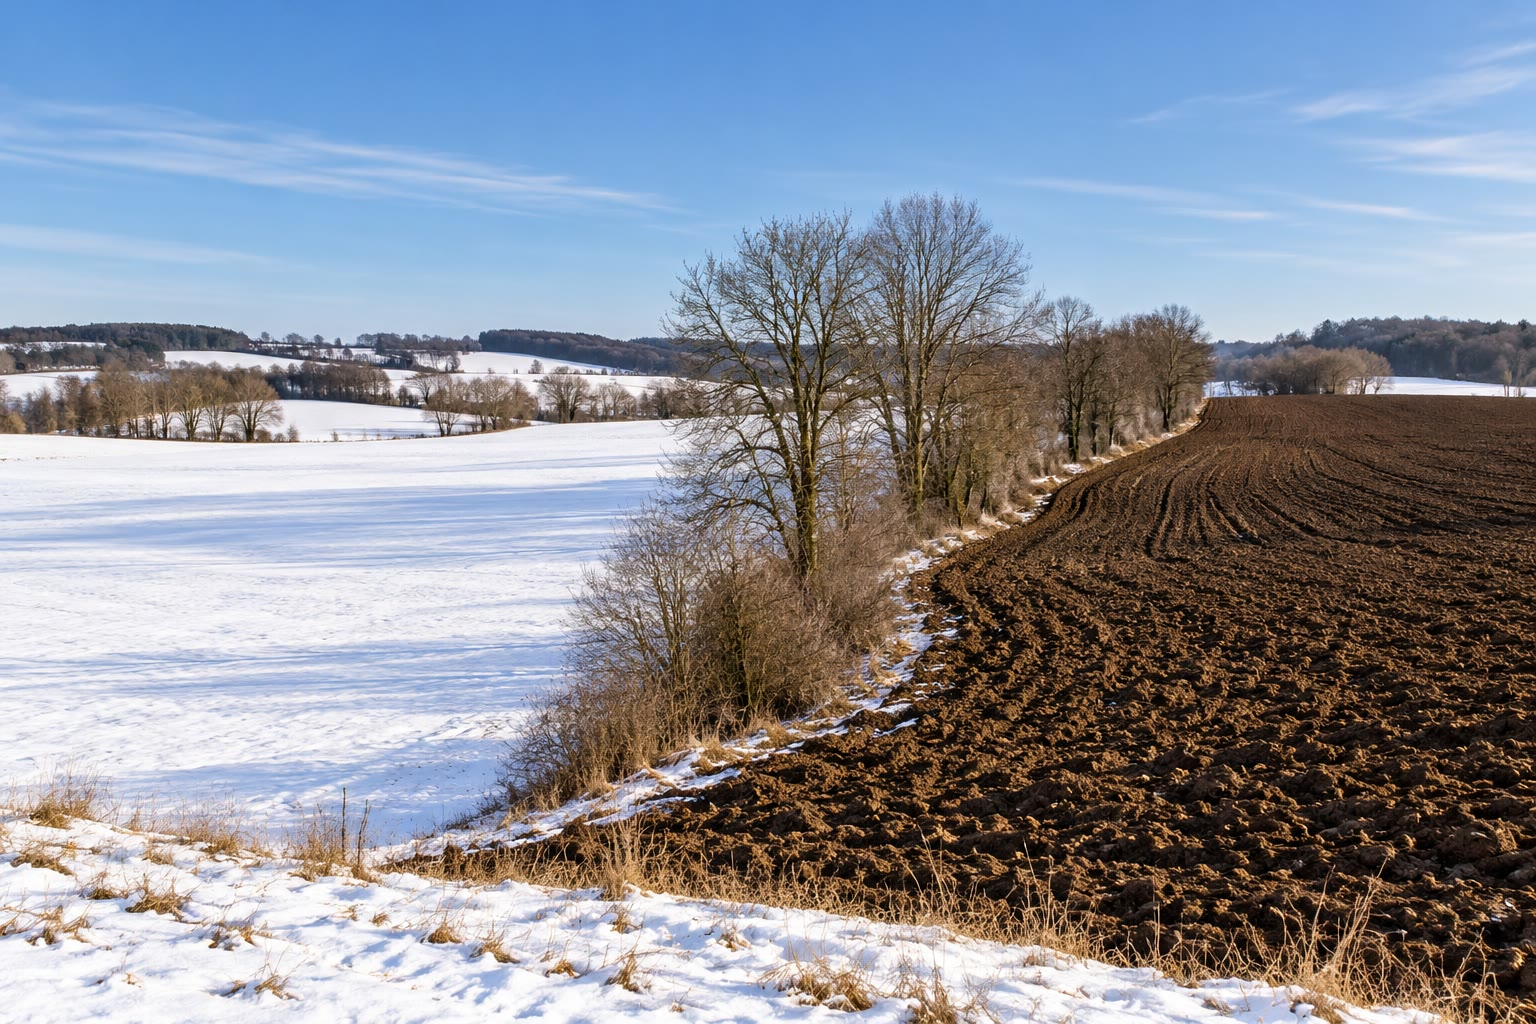
\includegraphics[width=0.7\linewidth]{images/book2/ai/g10-snow-and-ploughed-field.jpg}

{\small Uma manhã de inverno depois de alguns dias de sol: a neve ainda
cobre o prado, mas derreteu sobre o campo arado escuro, que absorve muito
mais luz solar.}
\end{omfigure}

Para a Terra como um todo, os satélites medem diretamente a luz solar
refletida para o espaço: em média \qty{100}{W/m^2} dos \qty{340}{W/m^2} que
chegam, um \omterm{def:g10:earth-energy-budget:albedo}{albedo} de $100/340 \approx 0.29$. As nuvens são o principal
refletor: as mesmas medidas, com as nuvens retiradas por cálculo, dão apenas
\qty{53}{W/m^2} refletidos.
% ledger: ipcc:budget-toa, ipcc:budget-clearsky, earth:albedo

\begin{example}[A luz solar que a Terra absorve]\label{ex:g10:earth-energy-budget:absorbed}
% ledger: earth:TSI, earth:albedo, earth:Rmean (computed in figdata/grade-10/energy_budget.py)
Com um \omterm{def:g10:earth-energy-budget:albedo}{albedo} de Bond de 0.294, cada metro quadrado absorve em média $340
\times (1 - 0.294) \approx \qty{240}{W/m^2}$. Sobre a esfera inteira, de
área $4\pi R^2 = 4\pi \times (\qty{6.371e6}{m})^2 \approx \qty{5.10e14}{m^2}$,
a Terra absorve $240 \times 5.10\times10^{14} \approx \qty{1.22e17}{W}$ de
luz solar: essa potência move os ventos, as correntes oceânicas e o ciclo
da água.
\end{example}

\section{O balanço global de energia}

Para onde vão esses \qty{240}{W/m^2}? Medidas feitas por satélites, por
instrumentos no chão e a bordo de navios, combinadas com modelos da
atmosfera, dão hoje uma resposta coerente, em média sobre o globo e sobre
vários anos. A avaliação científica de 2021 a resume no diagrama abaixo e
afirma que as componentes médias globais são hoje conhecidas com mais
exatidão, no topo da atmosfera e na superfície (\emph{alta confiança}).
% ledger: ipcc:budget-confidence

\begin{definition}[Balanço de energia]\label{def:g10:earth-energy-budget:energy-budget}
O \emph{balanço de energia}\index{balanco de energia@balanço de energia} de
um sistema --- a Terra inteira, a sua superfície ou a sua atmosfera --- é a
contabilidade de toda a energia que entra nele e sai dele, cada fluxo dado
como uma potência média por metro quadrado da superfície da Terra. O
balanço está \emph{equilibrado} quando o que entra é igual ao que sai; caso
contrário, o sistema ganha ou perde energia e se aquece ou se resfria.
\end{definition}

A superfície também perde energia sem nenhuma radiação: a água evapora do
mar e das folhas, e o chão aquece o ar em contato com ele.

\begin{definition}[Calor latente; calor sensível]\label{def:g10:earth-energy-budget:latent-heat}
O \emph{calor latente}\index{calor latente} de uma substância é a energia
que ela absorve quando muda de estado sem mudar de temperatura --- ao
fundir ou ao evaporar --- e que devolve quando volta ao estado anterior.
Para a água que evapora a \qty{15}{\degreeCelsius}, ele vale cerca de
\qty{2.47}{MJ} por quilograma. No \omterm{def:g10:earth-energy-budget:energy-budget}{balanço de energia}, o \emph{fluxo de calor
latente} é a energia que a evaporação retira da superfície e que o vapor de
água libera no ar onde se condensa em nuvens. O fluxo de
\emph{calor sensível}\index{calor sensivel@calor sensível} é a energia que a
superfície passa ao ar em contato com ela, aquecendo-o, e que o ar que sobe
leva para cima.
\end{definition}
% ledger: nist:water-latent

\begin{omfigure}
\begin{tikzpicture}[font=\footnotesize, >={Stealth[length=2.2mm, width=2mm]}, line width=1.4pt]
  % layers
  \fill[omDef!8] (0,0.5) rectangle (12.8,4.5);
  \fill[omExo!35] (0,0) rectangle (12.8,0.5);
  \draw[thin, black!60] (0,0.5) -- (12.8,0.5);
  \draw[thin, black!60, dashed] (0,4.5) -- (12.8,4.5);
  \node[anchor=east, black!70, align=right] at (-0.1,5.4) {espaço};
  \node[anchor=east, black!70, align=right] at (-0.1,4.5) {topo da\\atmosfera};
  \node[anchor=east, black!70, align=right] at (-0.1,2.5) {atmosfera};
  \node[anchor=east, black!70, align=right] at (-0.1,0.25) {superfície};
  \pic[scale=0.7, transform shape] at (4.3,3.0) {puffycloud};
  \pic[scale=0.7, transform shape] at (6.2,3.0) {puffycloud};
  % sunlight
  \draw[->, omProp!90!black] (1.0,6.1) -- (1.0,0.52);
  \draw[->, omProp!90!black] (1.0,3.0) -- (1.6,3.0);
  \node[anchor=west, align=left] at (1.65,3.0) {80 absorvidos\\pelo ar};
  \node[anchor=west] at (1.05,1.3) {185};
  \draw[->, omProp!55] (4.3,3.7) -- (4.3,6.1);
  \node[anchor=east] at (4.25,5.0) {75};
  \draw[->, omProp!55] (5.25,0.52) -- (5.25,6.1);
  \node[anchor=west] at (5.3,1.2) {25};
  % heat
  \draw[->, omMeth!80!black] (6.2,0.52) -- (6.2,2.95);
  \draw[->, omMeth!80!black] (7.8,0.52) -- (7.8,2.0);
  % infrared
  \draw[->, omThm!80!black] (9.2,0.52) -- (9.2,4.0);
  \draw[->, omThm!80!black] (10.7,3.4) -- (10.7,6.1);
  \draw[->, omThm!50] (12.1,4.0) -- (12.1,0.52);
  % words above the top of the atmosphere
  \node[anchor=south, align=center] at (1.0,6.15) {340\\incidentes};
  \node[anchor=south, align=center] at (4.78,6.15) {100\\refletidos};
  \node[anchor=south, align=center] at (7.7,5.0) {desequilíbrio\\$+0.7$ absorvidos};
  \node[anchor=south, align=center] at (10.7,6.15) {239 infraverm.\\para o espaço};
  % words below the surface
  \node[anchor=north, align=center] at (1.0,-0.05) {160\\absorvidos};
  \node[anchor=north, align=center] at (6.2,-0.05) {82\\calor\\latente};
  \node[anchor=north, align=center] at (7.8,-0.05) {21\\calor\\sensível};
  \node[anchor=north, align=center] at (9.4,-0.05) {398\\emitidos};
  \node[anchor=north, align=center] at (12.1,-0.05) {342\\radiação\\de retorno};
\end{tikzpicture}

{\small O balanço médio global de energia da Terra no início do
século~XXI, em \unit{W/m^2} médios sobre toda a superfície. Laranja: luz
solar; verde: calor levado pela evaporação e pelo ar quente; vermelho:
infravermelho. Dos 100 refletidos, 25 vêm da superfície e 75 das nuvens, do
ar e das suas poeiras. O infravermelho para o espaço inclui a parte da
emissão da superfície que escapa diretamente através do ar. Dados: IPCC,
Sexto Relatório de Avaliação, Grupo de Trabalho~I, Figura~7.2.}
\end{omfigure}
% ledger: ipcc:budget-toa, ipcc:budget-surface

\begin{method}[Ler um diagrama de balanço de energia]\label{met:g10:earth-energy-budget:reading}
\begin{enumerate}
  \item Escolha o sistema: a Terra inteira (uma linha acima da atmosfera),
        a superfície ou a atmosfera (a camada entre as duas).
  \item Liste as setas que entram nele e some-as; liste as setas que saem
        dele e some-as.
  \item Compare as duas somas. Se forem iguais, dentro do arredondamento
        dos números, o sistema está em equilíbrio; a diferença é o que ele
        ganha (ou perde) a cada segundo por metro quadrado.
\end{enumerate}
\end{method}

\begin{proposition}[O balanço fecha]\label{prop:g10:earth-energy-budget:balance}
Dentro do arredondamento dos valores, o balanço do diagrama acima está
equilibrado para a Terra como um todo, para a superfície e para a
atmosfera, com exceção de um pequeno excedente de cerca de
\qty{0.7}{W/m^2} que a Terra absorve e não devolve.
\end{proposition}

\begin{proof}
\emph{Terra inteira:} entram 340; saem $100 + 239 = 339$.
\emph{Superfície:} entram $160 + 342 = 502$; saem $82 + 21 + 398 = 501$. Nos
dois casos, o excedente, cerca de 1, é o desequilíbrio de 0.7 arredondado.
\emph{Atmosfera:} chame de $W$ a parte do infravermelho da superfície que
escapa através do ar para o espaço. O ar recebe
$80 + 82 + 21 + (398 - W) = 581 - W$ e emite $342$ para baixo e $239 - W$
para cima, $581 - W$ ao todo: equilibrado, qualquer que seja $W$.
\end{proof}
% ledger: ipcc:budget-toa, ipcc:budget-surface (closures checked in figdata/grade-10/energy_budget.py)

O diagrama também mostra o efeito estufa em ação. A superfície recebe do
ar, como infravermelho, \qty{342}{W/m^2} --- mais que o dobro da luz solar
que ela absorve, \qty{160}{W/m^2}. É por isso que ela pode emitir
\qty{398}{W/m^2}, a emissão de um corpo a cerca de \qty{15}{\degreeCelsius},
enquanto a Terra envia apenas \qty{239}{W/m^2} para o espaço. Os livros de
física constroem o modelo que liga esses números à temperatura; este livro
usa os fluxos medidos.

\begin{example}[Um metro de água por ano]\label{ex:g10:earth-energy-budget:evaporation}
% ledger: ipcc:budget-surface, nist:water-latent (computed in figdata/grade-10/energy_budget.py)
O fluxo de \omterm{def:g10:earth-energy-budget:latent-heat}{calor latente}, \qty{82}{W/m^2}, evapora a cada segundo
$82/2.47\times
10^6 \approx \qty{3.3e-5}{kg}$ de água por metro quadrado.
Em um ano, $3.16\times10^7$ segundos, isso dá cerca de \qty{1050}{kg}, uma
camada de água de \qty{1.05}{m} de espessura sobre a Terra inteira. O ar
só contém um pouco de água de cada vez, de modo que praticamente toda ela
volta a cair como chuva e neve: o fluxo de \omterm{def:g10:earth-energy-budget:latent-heat}{calor latente} e a chuva anual do
planeta são duas faces do mesmo ciclo da água.
\end{example}

\begin{remark}[O desequilíbrio]\label{rem:g10:earth-energy-budget:imbalance}
% ledger: ipcc:budget-toa, ipcc:heating
O excedente de \qty{0.7}{W/m^2} parece minúsculo ao lado de fluxos de
centenas de watts, mas sobre a Terra inteira ele dá $0.7 \times 5.10\times10^{14} \approx
\qty{3.6e14}{W}$, armazenados sobretudo no oceano,
que se aquece. Não é uma constante natural: ele cresceu nas últimas
décadas, como explica o \cref{ch:g12:climate-change}.
\end{remark}

\section{Excedente e déficit}

O balanço fecha para a Terra como um todo, mas não em cada latitude.

\begin{omfigure}
\begin{tikzpicture}
\begin{axis}[omrecord, width=0.86\linewidth, height=5.6cm, xmin=0, xmax=90,
  ymin=0, ymax=450, xlabel={latitude (\unit{\degree})},
  ylabel={insolação média anual (\unit{W/m^2})}, xtick={0,15,...,90},
  tick label style={font=\small}, label style={font=\small}]
\addplot[omThm!85!black, thick] table[x=lat, y=Qann] {figdata/out/grade-10-energy_budget-annual.dat};
\addplot[omDef!80!black, dashed, domain=0:90] {340.25};
\node[anchor=south west, font=\footnotesize, omDef!80!black] at (axis cs:2,343) {média global, 340};
\node[anchor=south west, font=\footnotesize, omThm!85!black] at (axis cs:62,232) {média anual};
\end{axis}
\end{tikzpicture}

{\small \omterm{def:g10:earth-energy-budget:insolation}{Insolação} média anual no topo da atmosfera em função da latitude
(a mesma nos dois hemisférios; calculada a partir da constante solar e da
inclinação do eixo). Entre o equador e cerca de \qty{37}{\degree}, ela
supera a média global; mais perto dos polos, fica abaixo dela.}
\end{omfigure}

Os trópicos absorvem muito mais luz solar que as regiões polares, e o seu
\omterm{def:g10:earth-energy-budget:albedo}{albedo} baixo aumenta a diferença. O infravermelho que eles enviam para o
espaço também é maior, porque eles são mais quentes, mas varia muito menos
com a latitude. Em consequência, as regiões em torno do equador absorvem
em média cerca de \qty{200}{W/m^2} a mais do que refletem e irradiam, e as
regiões perto dos polos irradiam cerca de \qty{200}{W/m^2} a mais do que
absorvem.
% ledger: nasaeo:surplus

\begin{definition}[Transporte de calor para os polos]\label{def:g10:earth-energy-budget:heat-transport}
O \emph{transporte de calor para os polos}\index{transporte de calor para os polos}
é o fluxo de energia levado dos trópicos em direção aos polos pelos
movimentos da atmosfera e do oceano. Ele é medido, através de um círculo de
latitude, em petawatts (\qty{1}{PW} = \qty{e15}{W}).
\end{definition}

Sem ele, os trópicos ficariam cada vez mais quentes e os polos cada vez
mais frios, até que cada latitude equilibrasse o seu próprio balanço. A
atmosfera faz a maior parte do transporte: ar quente que se desloca em
direção aos polos e ar frio que volta para o equador, e vapor de água que
libera o seu \omterm{def:g10:earth-energy-budget:latent-heat}{calor latente} longe de onde evaporou. As correntes oceânicas
levam o resto. Estimativas feitas a partir de medidas situam o máximo do
transporte atmosférico para os polos em cerca de \qty{5.0}{PW} perto de
\qty{43}{\degree} N, com valores semelhantes perto de \qty{40}{\degree} S; o
oceano só transporta mais que a atmosfera perto do equador, entre
\qty{0}{\degree} e \qty{17}{\degree} N, e a \qty{35}{\degree} N, onde o
transporte total é máximo, a atmosfera leva \qty{78}{\percent} dele. O
total é máximo ali porque \qty{35}{\degree} é mais ou menos onde o
excedente dá lugar ao déficit: em direção ao equador, o transporte vai
acumulando o excedente de cada latitude que atravessa; em direção ao polo,
cada latitude retira dele a sua parte.
% ledger: trenberth:transport

\begin{omfigure}
\begin{tikzpicture}[font=\footnotesize, >={Stealth[length=2mm]}]
  \def\R{2.4}
  \begin{scope}
    \clip (0,0) circle (\R);
    \fill[omThm!22] (-\R,{-\R*sin(35)}) rectangle (\R,{\R*sin(35)});
    \fill[omDef!22] (-\R,{\R*sin(35)}) rectangle (\R,\R);
    \fill[omDef!22] (-\R,-\R) rectangle (\R,{-\R*sin(35)});
  \end{scope}
  \draw[thick] (0,0) circle (\R);
  \draw[black!50] (-\R,0) -- (\R,0);
  \foreach \s in {1,-1} \draw[black!40, dashed] ({-\R*cos(35)},{\s*\R*sin(35)}) -- ({\R*cos(35)},{\s*\R*sin(35)});
  \node at (0,0.45) {excedente};
  \node at (0,1.95) {déficit};
  \node at (0,-1.95) {déficit};
  \node[anchor=west, black!60] at (\R+0.05,0) {equador};
  \node[anchor=west, black!60] at ({\R*cos(35)+0.05},{\R*sin(35)}) {\qty{35}{\degree} N};
  \node[anchor=west, black!60] at ({\R*cos(35)+0.05},{-\R*sin(35)}) {\qty{35}{\degree} S};
  \foreach \s in {1,-1} {
    \draw[->, very thick, omProp!90!black] ({-(\R+0.35)*cos(10)},{\s*(\R+0.35)*sin(10)}) arc ({180-10*\s}:{180-70*\s}:{\R+0.35});
    \draw[->, thick, omMeth!80!black] ({-(\R-0.45)*cos(8)},{\s*(\R-0.45)*sin(8)}) arc ({180-8*\s}:{180-55*\s}:{\R-0.45});
  }
  \node[anchor=east, omProp!90!black, align=right] at (-\R-0.75,1.6) {atmosfera};
  \node[anchor=east, omProp!90!black, align=right] at (-\R-0.75,-1.6) {atmosfera};
  \node[omMeth!80!black] at (-1.25,0.62) {oceano};
  \node[omMeth!80!black] at (-1.25,-0.62) {oceano};
\end{tikzpicture}

{\small Entre cerca de \qty{35}{\degree} S e \qty{35}{\degree} N, a Terra
absorve mais energia do que irradia; além dessas latitudes, em direção aos
polos, ela irradia mais do que absorve. A atmosfera (laranja) e o oceano
(verde) levam o excedente para os polos. Esquema: as larguras das setas não
estão em escala.}
\end{omfigure}

Esse transporte é o motor do tempo. As células de convecção e os ventos
globais do Livro 1, as tempestades do \cref{ch:g10:storms-and-cyclones} e
as grandes correntes oceânicas do \cref{ch:g10:layered-ocean} levam todos o
calor de onde o Sol dá demais para onde ele dá de menos.

\section{Para onde vai a energia}

Quase toda a energia da luz solar que a Terra absorve acaba como calor: ela
aquece o chão, o mar e o ar, evapora a água, move os ventos e as correntes,
e sai de novo como luz infravermelha. Uma parte minúscula segue outro
caminho: a fotossíntese a armazena nas ligações químicas dos açúcares e,
dali, em toda a matéria viva do planeta.

\begin{example}[A parte da fotossíntese]\label{ex:g10:earth-energy-budget:photosynthesis}
% ledger: field:npp, nist:glucose-combustion, earth:Rmean (computed in figdata/grade-10/energy_budget.py)
As plantas em terra e as algas no mar armazenam, depois das suas próprias
necessidades, cerca de \num{105} bilhões de toneladas de carbono em nova
matéria viva a cada ano, mais ou menos metade em terra e metade no oceano:
os ecólogos chamam isso de produção primária líquida do planeta. Queimar um
mol de glicose, \ce{C6H12O6}, que contém seis mols de carbono,
\qty{72}{g}, libera \qty{2805}{kJ}: cerca de \qty{38.9}{kJ} por grama de
carbono. A energia armazenada a cada ano é
$1.049\times10^{17}\,\unit{g} \times \qty{38.9e3}{J/g} \approx
\qty{4.1e21}{J}$, uma potência de $4.1\times10^{21}/3.16\times10^{7} \approx
\qty{1.3e14}{W}$. Comparada com os \qty{1.22e17}{W} de luz solar que a Terra
absorve, isso é cerca de \qty{0.1}{\percent}.
\end{example}

\begin{remark}[Uma parte pequena, um papel grande]\label{rem:g10:earth-energy-budget:life}
Um milésimo da luz solar absorvida alimenta quase toda a vida da Terra, e os
restos de plantas e algas enterrados ao longo de centenas de milhões de anos
formam o carvão, o petróleo e o gás natural
(\cref{ch:g11:fossil-fuel-geology}). O resto da luz solar --- mais de 99.9
por cento --- mantém o planeta quente e o seu ar, a sua água e o seu tempo
em movimento.
\end{remark}

\section{Exercícios}

\begin{exercise}[$\star$]\label{exo:g10:earth-energy-budget:1}
Defina a \omterm{def:g10:earth-energy-budget:insolation}{insolação} de um lugar e o \omterm{def:g10:earth-energy-budget:albedo}{albedo} de uma superfície. Qual reflete a
maior fração da luz solar, a neve fresca ou o oceano aberto?
\end{exercise}

\begin{exercise}[$\star$]\label{exo:g10:earth-energy-budget:2}
Usando o diagrama do \omterm{def:g10:earth-energy-budget:energy-budget}{balanço de energia} deste capítulo, dê, em porcentagem
dos \qty{340}{W/m^2} que chegam ao topo da atmosfera, a parte refletida para
o espaço, a parte absorvida pelo ar e a parte absorvida pela superfície.
\end{exercise}

\begin{exercise}[$\star$]\label{exo:g10:earth-energy-budget:3}
Um sol de verão fornece \qty{800}{W/m^2} ao chão. Que potência absorve um
metro quadrado coberto de asfalto novo (\omterm{def:g10:earth-energy-budget:albedo}{albedo} 0.04), e de neve fresca
(\omterm{def:g10:earth-energy-budget:albedo}{albedo} 0.85)?
\end{exercise}

\begin{exercise}[$\star$]\label{exo:g10:earth-energy-budget:4}
O que leva mais energia para longe da superfície da Terra: a evaporação ou
o aquecimento do ar em contato com o chão? Descreva em duas frases como a
energia retirada do mar pela evaporação chega ao ar lá no alto.
\end{exercise}

\begin{exercise}[$\star$]\label{exo:g10:earth-energy-budget:5}
Explique por que a \omterm{def:g10:earth-energy-budget:insolation}{insolação} média diária é nula no Polo Norte em dezembro
e dê a latitude além da qual isso acontece no solstício de dezembro.
\end{exercise}

\begin{exercise}[$\star\star$]\label{exo:g10:earth-energy-budget:6}
Usando a \cref{prop:g10:earth-energy-budget:height}, calcule a potência
recebida por um metro quadrado horizontal no topo da atmosfera quando o Sol
está a \qty{90}{\degree}, \qty{30}{\degree} e \qty{10}{\degree} acima do
horizonte. A que altura do Sol o metro quadrado recebe a metade de $S_0$?
\end{exercise}

\begin{exercise}[$\star\star$]\label{exo:g10:earth-energy-budget:7}
Seguindo o \cref{met:g10:earth-energy-budget:reading}, verifique o balanço
apenas da luz solar: dos \qty{340}{W/m^2} que chegam, quanto é refletido,
absorvido pelo ar e absorvido pela superfície? Os três somam 340? Verifique
também que a luz solar que chega à superfície, \qty{185}{W/m^2}, é ali
refletida ou absorvida.
\end{exercise}

\begin{exercise}[$\star\star$]\label{exo:g10:earth-energy-budget:8}
Com o raio médio da Terra, \qty{6371}{km}, calcule a área do disco que
intercepta a luz solar e a potência que ele intercepta e, depois, a área da
esfera. Deduza a potência média por metro quadrado da esfera.
\end{exercise}

\begin{exercise}[$\star\star$]\label{exo:g10:earth-energy-budget:9}
O excedente da Terra é de \qty{0.7}{W/m^2} sobre uma área de
\qty{5.10e14}{m^2}. Quanta energia, em joules, a Terra ganha num ano de
$3.16\times10^7$ segundos?
\end{exercise}

\begin{exercise}[$\star\star$]\label{exo:g10:earth-energy-budget:10}
Com as nuvens retiradas por cálculo, a Terra refletiria \qty{53}{W/m^2} em
vez de \qty{100}{W/m^2} e enviaria \qty{267}{W/m^2} de infravermelho para o
espaço em vez de \qty{239}{W/m^2}. Quanto as nuvens mudam a luz solar
absorvida e o infravermelho perdido? No saldo, as nuvens aquecem ou
resfriam a Terra?
\end{exercise}

\begin{exercise}[$\star\star$]\label{exo:g10:earth-energy-budget:11}
Leia as curvas de \omterm{def:g10:earth-energy-budget:insolation}{insolação} média diária deste capítulo. Em que meses a
\omterm{def:g10:earth-energy-budget:insolation}{insolação} média diária no Polo Norte é maior que no equador? Por que a
curva do equador mostra dois máximos e não um só?
\end{exercise}

\begin{exercise}[$\star\star\star$]\label{exo:g10:earth-energy-budget:12}
O \omterm{def:g10:earth-energy-budget:latent-heat}{calor latente} de evaporação da água é de \qty{2.47}{MJ/kg} e o fluxo de
\omterm{def:g10:earth-energy-budget:latent-heat}{calor latente}, de \qty{82}{W/m^2}. Calcule a espessura de água, em
milímetros, evaporada do metro quadrado médio da Terra a cada dia, e em
metros a cada ano (um litro de água espalhado sobre um metro quadrado forma
uma camada de \qty{1}{mm} de espessura).
\end{exercise}

\begin{exercise}[$\star\star\star$]\label{exo:g10:earth-energy-budget:13}
No Polo Norte, o Sol dá a volta no céu a uma altura igual à sua declinação
$\delta$, de modo que a \omterm{def:g10:earth-energy-budget:insolation}{insolação} média diária ali é $S_0 \sin
\delta$.
Encontre a declinação para a qual o polo recebe, em média sobre o dia,
tanto quanto o equador num equinócio, $S_0/\pi$. A declinação obedece a
$\sin\delta = \sin 23.44^\circ \times \sin\lambda$, em que o ângulo
$\lambda$ cresce regularmente \qty{360}{\degree} por ano, a partir de
\qty{0}{\degree} no equinócio de março (\qty{90}{\degree} no solstício de
junho). Durante aproximadamente quantos dias por ano o polo recebe mais que
$S_0/\pi$?
\end{exercise}

\begin{exercise}[$\star\star\star$]\label{exo:g10:earth-energy-budget:14}
Suponha que, no verão, uma área de \qty{1e12}{m^2} de gelo marinho (\omterm{def:g10:earth-energy-budget:albedo}{albedo}
0.6) derreta e seja substituída por oceano aberto (\omterm{def:g10:earth-energy-budget:albedo}{albedo} 0.06), sob uma luz
solar de \qty{300}{W/m^2} em média na superfície. Calcule a potência
absorvida a mais. Compare-a com a potência armazenada por toda a
fotossíntese da Terra, \qty{1.3e14}{W}, e explique por que essa troca de
superfícies se reforça a si mesma.
\end{exercise}

\begin{exercise}[$\star\star\star$]\label{exo:g10:earth-energy-budget:15}
A distância da Terra ao Sol é de \num{147.1} milhões de quilômetros no
ponto mais próximo e de \num{152.1} milhões no mais afastado, para uma média
de \num{149.6} milhões, onde $S_0 = \qty{1361}{W/m^2}$. Calcule a
irradiância solar nos dois extremos. A diferença é de cerca de
\qty{90}{W/m^2}; a \qty{60}{\degree} N, a \omterm{def:g10:earth-energy-budget:insolation}{insolação} média diária é de cerca
de \qty{490}{W/m^2} em junho e de \qty{24}{W/m^2} em dezembro. Explique por
que a distância não pode ser a causa das estações.
\end{exercise}

\section{Problema: seguindo um raio de sol}

\begin{problem}[{Problema de fim de semana --- da luz solar que chega à Terra
à parte que a vida armazena}]
\label{pb:g10:earth-energy-budget:1}
% ledger: earth:TSI, earth:Rmean, ipcc:budget-toa, ipcc:budget-surface, ipcc:budget-clearsky, nist:water-latent, field:npp, nist:glucose-combustion (all results computed in figdata/grade-10/energy_budget.py or from the rounded data below)
Use $S_0 = \qty{1361}{W/m^2}$, o raio da Terra $R = \qty{6371}{km}$,
$\sigma = \qty{5.67e-8}{W.m^{-2}.K^{-4}}$, um ano de $3.156\times10^7$
segundos, os fluxos do diagrama do \omterm{def:g10:earth-energy-budget:energy-budget}{balanço de energia}, um \omterm{def:g10:earth-energy-budget:latent-heat}{calor latente} de
evaporação de \qty{2.47}{MJ/kg}, uma produção primária líquida global de
\num{104.9} bilhões de toneladas de carbono por ano e \qty{2805}{kJ}
liberados pela queima de um mol de glicose (\qty{72.07}{g} de carbono).

\medskip
\noindent\textbf{Parte I --- A geometria da luz solar.}
\begin{enumerate}
  \item Calcule a área do disco que intercepta a luz solar, $\pi R^2$, em
        metros quadrados.
  \item Calcule a potência da luz solar que ele intercepta.
  \item Calcule a área da superfície da Terra, $4\pi R^2$.
  \item Deduza a potência média que chega por metro quadrado do topo da
        atmosfera.
  \item Num equinócio, ao meio-dia, o Sol está a pino no equador e a
        \qty{30}{\degree} acima do horizonte a \qty{60}{\degree} N. O que
        recebe um metro quadrado horizontal em cada lugar?
\end{enumerate}

\medskip
\noindent\textbf{Parte II --- O albedo.}
\begin{enumerate}[resume]
  \item A partir dos \qty{100}{W/m^2} refletidos, calcule o \omterm{def:g10:earth-energy-budget:albedo}{albedo} da Terra.
  \item Calcule a potência absorvida por metro quadrado e pela Terra
        inteira.
  \item Sem nuvens, \qty{53}{W/m^2} seriam refletidos. Qual seria o \omterm{def:g10:earth-energy-budget:albedo}{albedo}?
        Por que fator as nuvens o aumentam?
  \item Calcule a \omterm{def:g10:habitable-planet:equilibrium-temperature}{temperatura de equilíbrio} correspondente à potência
        absorvida da questão 7 (\cref{ch:g10:habitable-planet}) e
        compare-a com os \qty{288}{K} da superfície.
\end{enumerate}

\medskip
\noindent\textbf{Parte III --- A superfície.}
\begin{enumerate}[resume]
  \item Some os fluxos de energia que entram na superfície.
  \item Some os que saem dela e compare.
  \item Quantas vezes maior que a luz solar absorvida pela superfície é o
        infravermelho que ela recebe do ar? O que isso mostra?
  \item Calcule a massa de água evaporada de um metro quadrado em um ano e
        a espessura da camada que ela forma.
  \item Calcule a potência total do desequilíbrio, \qty{0.7}{W/m^2}, sobre
        a Terra inteira.
\end{enumerate}

\medskip
\noindent\textbf{Parte IV --- A parte da vida.}
\begin{enumerate}[resume]
  \item Calcule a energia armazenada por grama de carbono fixado na
        glicose.
  \item Calcule a energia armazenada em um ano pela produção primária
        líquida.
  \item Converta-a numa potência.
  \item Expresse-a por metro quadrado da superfície da Terra.
  \item Compare-a com o desequilíbrio da questão 14.
  \item Que parte da luz solar absorvida pela Terra (questão 7) a
        fotossíntese armazena?
\end{enumerate}
\end{problem}
